
%% %%
%% %% INTRO
%% %%

\slide{ Recent updates }
{
wmunu version: v6:
\iteb
\item Switched from mu18\_MG (buggy) to mu18 trigger
\item Increased number of MC toys (for SFs) from 100 to 1000
\itee
wmunu version: v7:
\iteb
\item Fixed a bug that treated uncorrelated portion of QCD uncertainty as correlated
\item Added full difference between MET and W\_mT fits to QCD systematics
\item Wpt systematic updated to sum-in-quadrature of Sherpa14MC11 and PowhegPythia8MC11
\itee
wmunu version: v8: (\red{new})
\iteb
\item Pileup uncertainty (scaling $<mu>$ by 0.97)
\item New source of QCD uncertainty: difference in DtoM fit vs (DtoK+LtoM)
\itee
}


\slide{ Effect of latest changes }
{
Nominal values remain unchanged. \\
Systematic plots are shown below (and in backup). \\
Changes from v7 to v8 are very minor: focus on the QCD systematic curve. \\
Additional comments:
\iteb
\item Pileup uncertainty is insignificant, except for the lowest-pt bin (20-25 GeV)
\item Uncertainty on QCD is a lot larger in the single-differential case with $pt>20$ GeV
\item Wmunu channel does not suffer from large MET vs WMT fit differences, so the QCD systematic is smaller than Wenu
\itee
}

\slide{ Single-differential uncertainties ($pt>25$ GeV) }
{
\colb[T]
\column{.5\textwidth}
\centering
\only<1>{ \small{ $W^{-}$: wmunu v7} }
\only<2>{ \small{ $W^{-}$: wmunu v8} }
\includegraphics[width=1.0\textwidth]<1>{dates/20130602/figures/v26/Wmn_SYSTEM_1D_PT25_NEG_Unc_proj}
\includegraphics[width=1.0\textwidth]<2>{dates/20130602/figures/v26.allqcd/Wmn_SYSTEM_1D_PT25_NEG_Unc_proj}
\column{.5\textwidth}

\centering
\only<1>{ \small{ $W^{+}$: wmunu v7} }
\only<2>{ \small{ $W^{+}$: wmunu v8} }
\includegraphics[width=1.0\textwidth]<1>{dates/20130602/figures/v26/Wmn_SYSTEM_1D_PT25_POS_Unc_proj}
\includegraphics[width=1.0\textwidth]<2>{dates/20130602/figures/v26.allqcd/Wmn_SYSTEM_1D_PT25_POS_Unc_proj}
\cole
}

\slide{ Compare with: single-differential wenu ($pt>25$ GeV)}
{
\colb[T]
\column{.5\textwidth}
\centering
\small{ $W^{-}$: wenu}
\includegraphics[width=1.0\textwidth]{/home/antonk/SupportingDocument/Wenu/figures/uncert/with_theory/Wenu_Unc_neg}
\column{.5\textwidth}

\centering
\small{ $W^{+}$: wenu}
\includegraphics[width=1.0\textwidth]{/home/antonk/SupportingDocument/Wenu/figures/uncert/with_theory/Wenu_Unc_pos}
\cole
}

\slide{ Single-differential uncertainties ($pt>20$ GeV) }
{
\colb[T]
\column{.5\textwidth}
\centering
\only<1>{ \small{ $W^{-}$: wmunu v7} }
\only<2>{ \small{ $W^{-}$: wmunu v8} }
\includegraphics[width=1.0\textwidth]<1>{dates/20130602/figures/v26/Wmn_SYSTEM_1D_PT20_NEG_Unc_proj}
\includegraphics[width=1.0\textwidth]<2>{dates/20130602/figures/v26.allqcd/Wmn_SYSTEM_1D_PT20_NEG_Unc_proj}
\column{.5\textwidth}

\centering
\only<1>{ \small{ $W^{+}$: wmunu v7} }
\only<2>{ \small{ $W^{+}$: wmunu v8} }
\includegraphics[width=1.0\textwidth]<1>{dates/20130602/figures/v26/Wmn_SYSTEM_1D_PT20_POS_Unc_proj}
\includegraphics[width=1.0\textwidth]<2>{dates/20130602/figures/v26.allqcd/Wmn_SYSTEM_1D_PT20_POS_Unc_proj}
\cole
}

% TODO - add single-differential table from break-down folder

\slide{ Stat. uncertainty on scale factors: wmunu vs zmumu }
{
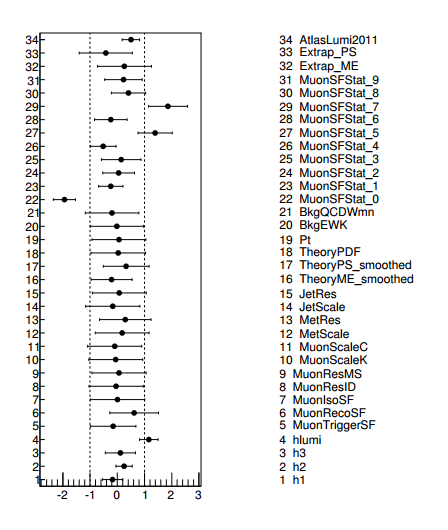
\includegraphics[width=0.4\textwidth]{dates/20130602/figures/fit/wmunu}
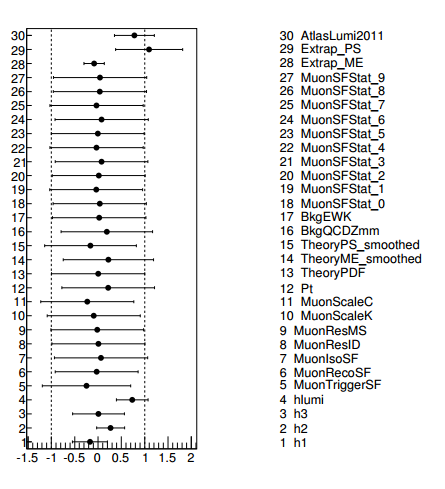
\includegraphics[width=0.4\textwidth]{dates/20130602/figures/fit/zmumu}
}

\slide{ Stat. uncertainty on scale factors: reco, trig, iso }
{
\includegraphics[width=1.0\textwidth]<1>{dates/20130602/figures/toysf/EVENT_8701402}
\includegraphics[width=1.0\textwidth]<2>{dates/20130602/figures/toysf/EVENT_8701405}
\includegraphics[width=1.0\textwidth]<3>{dates/20130602/figures/toysf/EVENT_8701409}
\includegraphics[width=1.0\textwidth]<4>{dates/20130602/figures/toysf/EVENT_8701411}
\includegraphics[width=1.0\textwidth]<5>{dates/20130602/figures/toysf/EVENT_8701412}
}

%%%%%%% Back-up slides %%%%%%%%%%
\appendix
\newcounter{finalframe}
\setcounter{finalframe}{\value{framenumber}}

\slide{}
{
\centering
\Huge Back-up slides
}

\slide{ Double-differential uncertainties }
{
Effect of latest updates on double-differential uncertainties. \\
Summary: appreciable change in the first and last $p_T$ bins; small elsewhere.
}

\slide{ $20 < p_T < 25$ }
{
\colb[T]
\column{.5\textwidth}
\centering
\only<1>{ \small{ $W^{-}$: wmunu v7} }
\only<2>{ \small{ $W^{-}$: wmunu v8} }
\includegraphics[width=1.0\textwidth]<1>{dates/20130602/figures/v26/Wmn_SYSTEM30_2D_PT20_NEG_Unc_2d_Slice_1}
\includegraphics[width=1.0\textwidth]<2>{dates/20130602/figures/v26.allqcd/Wmn_SYSTEM30_2D_PT20_NEG_Unc_2d_Slice_1}
\column{.5\textwidth}

\centering
\only<1>{ \small{ $W^{+}$: wmunu v7} }
\only<2>{ \small{ $W^{+}$: wmunu v8} }
\includegraphics[width=1.0\textwidth]<1>{dates/20130602/figures/v26/Wmn_SYSTEM30_2D_PT20_POS_Unc_2d_Slice_1}
\includegraphics[width=1.0\textwidth]<2>{dates/20130602/figures/v26.allqcd/Wmn_SYSTEM30_2D_PT20_POS_Unc_2d_Slice_1}
\cole
}

\slide{ $25 < p_T < 30$ }
{
\colb[T]
\column{.5\textwidth}
\centering
\only<1>{ \small{ $W^{-}$: wmunu v7} }
\only<2>{ \small{ $W^{-}$: wmunu v8} }
\includegraphics[width=1.0\textwidth]<1>{dates/20130602/figures/v26/Wmn_SYSTEM_2D_PT20_NEG_Unc_2d_Slice_2}
\includegraphics[width=1.0\textwidth]<2>{dates/20130602/figures/v26.allqcd/Wmn_SYSTEM_2D_PT20_NEG_Unc_2d_Slice_2}
\column{.5\textwidth}

\centering
\only<1>{ \small{ $W^{+}$: wmunu v7} }
\only<2>{ \small{ $W^{+}$: wmunu v8} }
\includegraphics[width=1.0\textwidth]<1>{dates/20130602/figures/v26/Wmn_SYSTEM_2D_PT20_POS_Unc_2d_Slice_2}
\includegraphics[width=1.0\textwidth]<2>{dates/20130602/figures/v26.allqcd/Wmn_SYSTEM_2D_PT20_POS_Unc_2d_Slice_2}
\cole
}

\slide{ $30 < p_T < 35$ }
{
\colb[T]
\column{.5\textwidth}
\centering
\only<1>{ \small{ $W^{-}$: wmunu v7} }
\only<2>{ \small{ $W^{-}$: wmunu v8} }
\includegraphics[width=1.0\textwidth]<1>{dates/20130602/figures/v26/Wmn_SYSTEM_2D_PT20_NEG_Unc_2d_Slice_3}
\includegraphics[width=1.0\textwidth]<2>{dates/20130602/figures/v26.allqcd/Wmn_SYSTEM_2D_PT20_NEG_Unc_2d_Slice_3}
\column{.5\textwidth}

\centering
\only<1>{ \small{ $W^{+}$: wmunu v7} }
\only<2>{ \small{ $W^{+}$: wmunu v8} }
\includegraphics[width=1.0\textwidth]<1>{dates/20130602/figures/v26/Wmn_SYSTEM_2D_PT20_POS_Unc_2d_Slice_3}
\includegraphics[width=1.0\textwidth]<2>{dates/20130602/figures/v26.allqcd/Wmn_SYSTEM_2D_PT20_POS_Unc_2d_Slice_3}
\cole
}

\slide{ $35 < p_T < 40$ }
{
\colb[T]
\column{.5\textwidth}
\centering
\only<1>{ \small{ $W^{-}$: wmunu v7} }
\only<2>{ \small{ $W^{-}$: wmunu v8} }
\includegraphics[width=1.0\textwidth]<1>{dates/20130602/figures/v26/Wmn_SYSTEM_2D_PT20_NEG_Unc_2d_Slice_4}
\includegraphics[width=1.0\textwidth]<2>{dates/20130602/figures/v26.allqcd/Wmn_SYSTEM_2D_PT20_NEG_Unc_2d_Slice_4}
\column{.5\textwidth}

\centering
\only<1>{ \small{ $W^{+}$: wmunu v7} }
\only<2>{ \small{ $W^{+}$: wmunu v8} }
\includegraphics[width=1.0\textwidth]<1>{dates/20130602/figures/v26/Wmn_SYSTEM_2D_PT20_POS_Unc_2d_Slice_4}
\includegraphics[width=1.0\textwidth]<2>{dates/20130602/figures/v26.allqcd/Wmn_SYSTEM_2D_PT20_POS_Unc_2d_Slice_4}
\cole
}

\slide{ $40 < p_T < 45$ }
{
\colb[T]
\column{.5\textwidth}
\centering
\only<1>{ \small{ $W^{-}$: wmunu v7} }
\only<2>{ \small{ $W^{-}$: wmunu v8} }
\includegraphics[width=1.0\textwidth]<1>{dates/20130602/figures/v26/Wmn_SYSTEM_2D_PT20_NEG_Unc_2d_Slice_5}
\includegraphics[width=1.0\textwidth]<2>{dates/20130602/figures/v26.allqcd/Wmn_SYSTEM_2D_PT20_NEG_Unc_2d_Slice_5}
\column{.5\textwidth}

\centering
\only<1>{ \small{ $W^{+}$: wmunu v7} }
\only<2>{ \small{ $W^{+}$: wmunu v8} }
\includegraphics[width=1.0\textwidth]<1>{dates/20130602/figures/v26/Wmn_SYSTEM_2D_PT20_POS_Unc_2d_Slice_5}
\includegraphics[width=1.0\textwidth]<2>{dates/20130602/figures/v26.allqcd/Wmn_SYSTEM_2D_PT20_POS_Unc_2d_Slice_5}
\cole
}

\slide{ $45 < p_T < 50$ }
{
\colb[T]
\column{.5\textwidth}
\centering
\only<1>{ \small{ $W^{-}$: wmunu v7} }
\only<2>{ \small{ $W^{-}$: wmunu v8} }
\includegraphics[width=1.0\textwidth]<1>{dates/20130602/figures/v26/Wmn_SYSTEM_2D_PT20_NEG_Unc_2d_Slice_6}
\includegraphics[width=1.0\textwidth]<2>{dates/20130602/figures/v26.allqcd/Wmn_SYSTEM_2D_PT20_NEG_Unc_2d_Slice_6}
\column{.5\textwidth}

\centering
\only<1>{ \small{ $W^{+}$: wmunu v7} }
\only<2>{ \small{ $W^{+}$: wmunu v8} }
\includegraphics[width=1.0\textwidth]<1>{dates/20130602/figures/v26/Wmn_SYSTEM_2D_PT20_POS_Unc_2d_Slice_6}
\includegraphics[width=1.0\textwidth]<2>{dates/20130602/figures/v26.allqcd/Wmn_SYSTEM_2D_PT20_POS_Unc_2d_Slice_6}
\cole
}

\slide{ $p_T > 50$ }
{
\colb[T]
\column{.5\textwidth}
\centering
\only<1>{ \small{ $W^{-}$: wmunu v7} }
\only<2>{ \small{ $W^{-}$: wmunu v8} }
\includegraphics[width=1.0\textwidth]<1>{dates/20130602/figures/v26/Wmn_SYSTEM_2D_PT20_NEG_Unc_2d_Slice_7}
\includegraphics[width=1.0\textwidth]<2>{dates/20130602/figures/v26.allqcd/Wmn_SYSTEM_2D_PT20_NEG_Unc_2d_Slice_7}
\column{.5\textwidth}

\centering
\only<1>{ \small{ $W^{+}$: wmunu v7} }
\only<2>{ \small{ $W^{+}$: wmunu v8} }
\includegraphics[width=1.0\textwidth]<1>{dates/20130602/figures/v26/Wmn_SYSTEM_2D_PT20_POS_Unc_2d_Slice_7}
\includegraphics[width=1.0\textwidth]<2>{dates/20130602/figures/v26.allqcd/Wmn_SYSTEM_2D_PT20_POS_Unc_2d_Slice_7}
\cole
}
